\documentclass{beamer}
\usetheme{Singapore}
\usecolortheme{rose}
\usefonttheme{serif}
\usepackage[latin1]{inputenc}
\usepackage{graphicx}
\usepackage{algpseudocode}
\setbeamertemplate{navigation symbols}{}

%Use only when printing
%usepackage{pgfpages}
%\pgfpagesuselayout{resize to}[a4paper,border shrink=5mm,landscape]
%Uncomment the above 2 lines when making a pdf to print, for the presentation use a pdf compiled with them commented out

\author{David Kroukamp (536705)\\and\\Wade Pimenta (544147)}
\title{HPC - Assignment 2\\CUDA}
\institute{University of the Witwatersrand, Johannesburg,
South Africa}
\date{\today}

\begin{document}
\begin{frame}
	\maketitle
\end{frame}

\begin{frame}
	\frametitle{Outline}
	\tableofcontents
\end{frame}

\section{Introduction}
\subsection{Problem Description}
\begin{frame}
	\frametitle{Problem Description}
	1D heat diffusion is the diffusion of heat along an infinitely narrow pipe. Initially, the whole pipe is at a stable and fixed temperature; for clarity purposes, we set our pipes initial temperature to be zero. At the start (time 0), we set both ends to a specified temperature, which remains fixed through the computation. We then calculate how the temperatures change in the rest of the pipe over time. Mathematically, the problem is to solve a 1D differential equation representing heat diffusion:
	$$\frac{\delta u}{\delta t} = \frac{\delta^{2}u}{\delta x^{2}}$$
\end{frame}
\begin{frame}
	\frametitle{Problem Description (cont.)}
	Our approach is to discretize the problem space by representing $U$ by a one-dimensional array and computing values for a sequence of discrete time steps. Assume we have the values for $U$ at time step $k$ in an array $Uk$, then for the next time step $k + 1$ update the second array $Ukp1$ as
	$$Ukp1[i] = Uk[i] + \frac{dt}{dx \times dx}(Uk[i+1] - 2Uk[i] + Uk[i-1])$$ where $dt$ and $dx$ represents the intervals between discrete time steps and between discrete points respectively.
\end{frame}

\section{A Visual Representation}
\begin{frame}
	\frametitle{A Visual Representation}
	The following is a visual representation of the update function $$Ukp1[i] = Uk[i] + \frac{dt}{dx \times dx}(Uk[i+1] - 2Uk[i] + Uk[i-1])$$
	\begin{figure}
		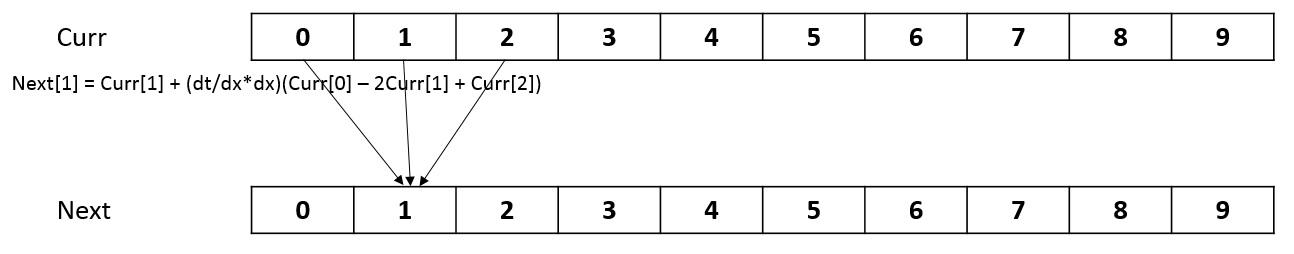
\includegraphics[width=11cm]{Visual1.jpg}
	\end{figure}
\end{frame}

\begin{frame}
	\frametitle{A Visual Representation (cont.)}
	\begin{figure}
		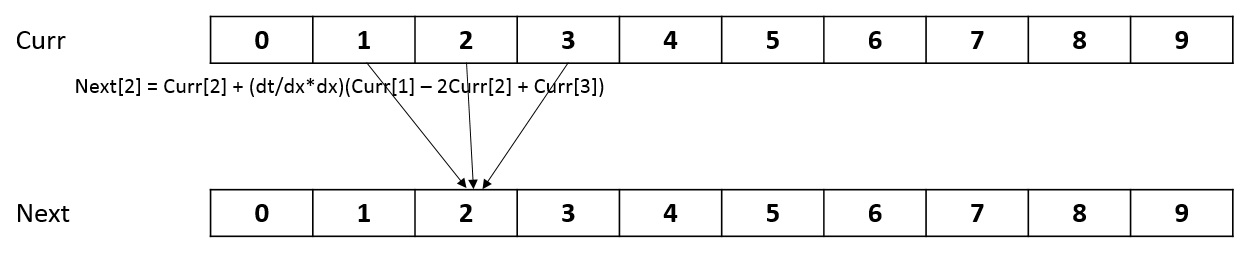
\includegraphics[width=11cm]{Visual2.jpg}
	\end{figure}
	\bigskip
	\begin{figure}
		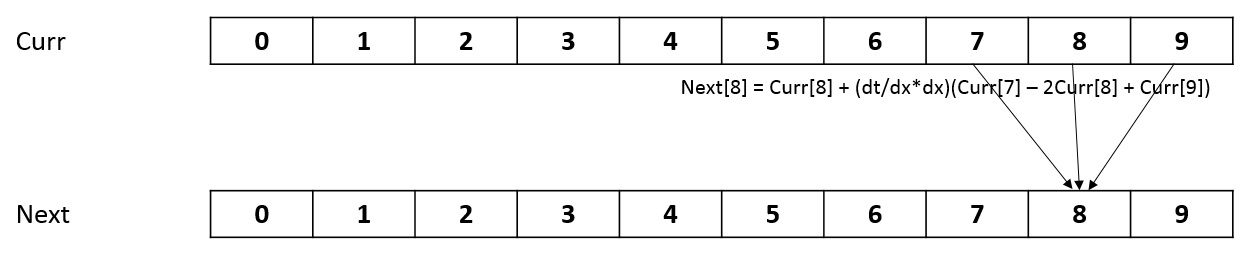
\includegraphics[width=11cm]{Visual3.jpg}
	\end{figure}
\end{frame}

\section{The CUDA Implementation}
\begin{frame}
	\frametitle{The CUDA Implementation}
	Visually, we can see that the calculation of each new element can be done at the same time as the other elements since there are no data dependencies.\\
	We can apply the following algorithm:\\
	\begin{algorithmic}
		\If {$\text{(tIdx \textgreater 0 and tIdx \textless arraySize-1)}$}
		\While {$\text{currentTime \textless endTime}$}
		\State $nextArray[tIdx] \gets currentArray[tIdx] + 0.25(currentArray[tIdx-1]$\\$-2*currentArray[tIdx] + currentArray[tIdx])$
		\State $\text{Sync threads and copy contents of nextArray to currentArray}$
		\State $\text{Increment currentTime by timestep}$		
		\EndWhile
		\EndIf
	\end{algorithmic}
\end{frame}

\begin{frame}
	\frametitle{The Code}
	\begin{figure}
		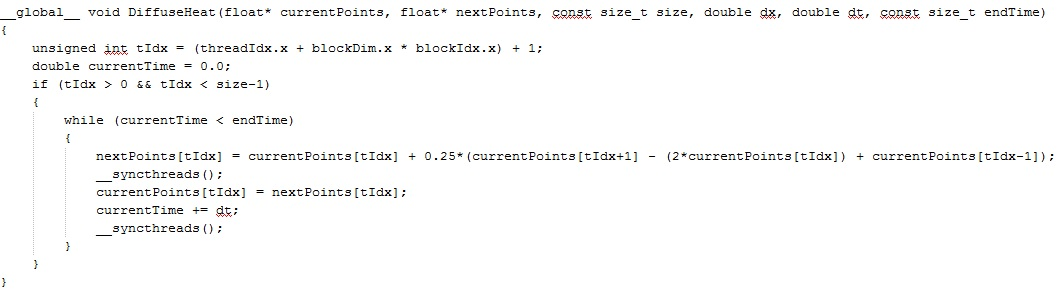
\includegraphics[width=11cm]{cudacode.jpg}
	\end{figure}
\end{frame}

\end{document}
